%%% Document Author: J Moss
%%% Parts in LaTeX: Nicholas Dart
%%% Other Content: See authors list
%%% Document Last edit: 28.10.2014

\documentclass[11pt, article]{article}
\usepackage{a4wide}
\usepackage[english]{babel}
\usepackage{graphicx}
\usepackage{tabu}
\usepackage{textcomp}
\usepackage{fancyhdr}
\usepackage{lastpage}
\usepackage{titlesec}
\usepackage{lscape}
\usepackage{longtable}
\usepackage{fixltx2e}
\usepackage[T1]{fontenc}
\usepackage[toc,page]{appendix}

%%%%%%
%% Variables for version and release status
%% useage: \version
%%%%%%
\newcommand\module{CS25410}
\newcommand\titleText{Development of Digital Circuits}
\newcommand\authorText{Nicholas Dart (nid21)}
\newcommand\assesser{Thomas Jansen}

%%%%%%
%% Alias
%%%%%%
%%\newcommand{\sectionbreak}{\clearpage}    %% Allways start a section on a new page
%% Never worked anyway...
%% ]\newcommand{\figureRef[x]{i}{d}{l}}{\begin{figure} \centering \includegraphics[scale=x]{i} \caption{d} \label{fig:l} \end{figure}}

\title{ \huge \module Project \\ \Large \titleText}
\author{
    \vspace{100pt}
    \begin{tabular}{ r || l }
        Author          & \authorText \\
        Date Published  & \today \\
                        & \\
        Assessed By     & \assesser \\
        Department      & Computer Science \\
        Address         & Aberystwyth University \\
                        & Penglais Campas \\
                        & Ceredigion \\
                        & SY23 3DB \\
    \end{tabular} \\
    Copyright \textcopyright Aberystwyth University 2014
    %get rid of the date on the titlepage
    \date{}
}

\pagestyle{fancy}
\fancyhf{}
\lhead{\module: \titleText}
\rhead{\authorText}
\rfoot{Page \thepage \hspace{1pt} of \pageref{LastPage}}
\lfoot{Aberystwyth University - Computer Science}

\begin{document}

    \maketitle
    \thispagestyle{empty}
    \newpage

    \setcounter{page}{1} %%Start counting pages from TOC
    \tableofcontents
    \newpage

    \section{Introduction}
        The task set forth in the assignment document requires me to implement a three bit comparator, internally containing two 3-bit registers which are capable of counting the number of rising edges on their respective inputs. The inputs are labeled as `A' and `B' in the spec and the registers are labeled as `a' and `b' in the specification, and for continuity will be referred to here as the same. The spec also defines a third input `R' whose job is to rest the internal counters to zero, and two outputs of the circuit; `E' and `G'. `E' is high (true) if either counter `a' or `b' holds the value 7 and `G' is high if the value stored in `a' is greater than the value in `b' and neither `a' nor `b' are equal to seven. In the context of the specification, i have determined ``if a or b'' to mean the logical or (IE one, the other, or both). 

    \section{Overview of Design}
        \subsection{Structure}
            The circuit requirements set forth in the specification have three main components to them:
            \begin{itemize}
                \item A three bit register, capable of counting the number of rising edges from a single input source
                \item An output capable of detecting if the register `a' or `b' store the value of 7
                \item An output capable of detecting if the register `a' is greater in value than `b' and neither `a' nor `b' are equal to 7
            \end{itemize}

        \subsection{Interesting Features/Shortcuts}
            The nature of the task provides some ways to reduce the number of gates used. For example the output of `E' can be negated and used as part of the comparison between `a' and `b'.

        \subsection{Initial Design Plans}
            \subsubsection{Register Comparison}
                \label{sec:register}
                My initial designs for an `A' > `B' comparator were as follows:
                \begin{itemize}
                    \item If a\textsubscript{n} is true and b\textsubscript{n} is false, and any more significant bitwise comparisons are equal, then any less significant bits are irrelevant, `A' is larger
                    \item If a\textsubscript{n} is equal to b\textsubscript{n} then proceed to the next bitwise comparison
                    \item If a\textsubscript{n} is false and b\textsubscript{n} is true, and any more significant bitwise comparisons are equal, then any less significant bits are irrelevant, `B' is larger
                \end{itemize}
                Where x\textsubscript{n} is register x, bit n.\\
                This approach is simple for a single bitwise comparison, requiring on only an AND gate and the register output (and inverted output). The approach should then be scalable bitwise with only the addition of a bigger input AND gate for checking bitwise x\textsubscript{n-1} are equal (where n-1 is a more significant bit)

            \subsubsection{`a' OR `b' equal seven}
                \label{sec:equal}
                This subsystem consists of a simply AND-ing all the outputs of a register to determine if the value is seven (seven in binary is 0b111) and then OR-ing the output of the AND from each register. This will determine if either `a', `b' or both are equal to seven.

    \section{Choice of Flip-Flops}
        My choice of flip-flops is two fold: I have a large amount of experience working with D-Type flip-flops from GCSE and A-Level Electronics courses and so have made counters and registers with them. However the primary reason for my choice is they provide a concise and simple way to implement counters. A D-Type can be set up so it's data value `D' is the inverted output `$\overline{Q}$' This ensures it always toggles it's state, thus creating a simple one-bit counter. These one-bit counters can then be daisy-chained to create larger counters if subsequent counters clock on `$\overline{Q}$' of the previous D-Type. Clocking on `$\overline{Q}$' is required to count up, locking on `Q' will count down.

    \section{Implementation}        
        \subsection{Registers}
            As described in my design for the registers (see section~\ref{sec:register}) I have quite a bit of experience working with D-type latches, and so the design for the counter was one I had used several times. The final counter used in the system required no alterations to the design (see appendix~\ref{fig:counter})

        \subsection{Comparator}
            The one-bit comparator I described in section \ref{sec:register} worked as designed, and and on scaling to three bits worked largely as designed. However In implementation I realized that the design could be simplified to require fewer gates. By changing the preconditions of success, I can achieve the same result: rather than having a `b\textsubscript{n}' is greater than `a\textsubscript{n}' compilation, I instead inverting it and including it in the `a\textsubscript{n}' greater than `b\textsubscript{n}' (see appendix~\ref{fig:system})

    \section{Conclusion}
        Testing of the system seems to indicate it preforms all the required tasks. However I believe my solution to be inefficient and rudimentary. Whilst it is likely that a decision on if `a' is greater than `b' is likely to be reached after checking only a few bits, for systems with larger registers this approach is likely impractical. In theory this approach could be made more parallel by computing a computing bitwise operations in pairs simultaneously (eg for a 32 bit system. compute 16 sets of `two bit registers' and then trickle down until a decision is reached) However I still believe my solution to be slow as for large registers there will likely be a high depth to the circuit.

    \section{Appendices}
        \begin{figure}
            \centering
                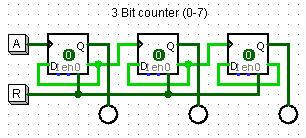
\includegraphics[scale=1]{counter.png}
            \caption{A simple one-bit counter}
            \label{fig:counter}
        \end{figure}

        \begin{figure}
            \centering
                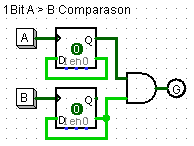
\includegraphics[scale=1]{comparitor.png}
            \caption{A Simple three-bit comparator}
            \label{fig:comparator}
        \end{figure}

        \begin{landscape}
            \begin{figure}
                \centering
                    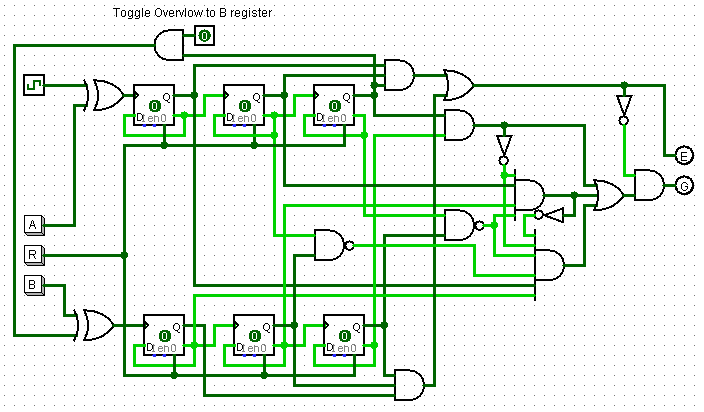
\includegraphics[scale=1]{system.png}
                \caption{The completed System}
                \label{fig:system}
            \end{figure}
        \end{landscape}

\end{document}